\title{First Flight of the EUV Snapshot Imaging Spectrograph (ESIS)}

\begin{abstract}
    This is the abstract.
\end{abstract} 

\section{Introduction}
    \begin{itemize}
        \item Instrument Heritage
            Brief summary since this is a repeat of the instrument paper.
        \item Scientific Motivation and Goals
            There is A LOT of this copied from the proposal into the instrument paper.  I think it needs to be lightly summarized here.
        \item Sections Outline
    \end{itemize}
    

\section{ESIS Mission}
    \begin{itemize}
        \item Brief description of the instrument, mostly pointing to the instrument paper.  Describe ESIS enough so that the data levels make sense. Need to consult the instrument paper to see what fits here. 
        \item ESIS Flight info.  Time, airtime, pointing, stability, etc.  Suggestions welcome here.
        \item Summary of Coordinated Data????
    \end{itemize}
    
\subsection{The Experiment}
Description of the instrument/camera, point to the instrument paper
    
\subsection{Flight Performance} \label{sec:flt}

ESIS was launched at ????~UT on September 30, 2019 from White Sands Missile Range.  The target of observation was quiet sun at disk center.  The Solar Pointing and Aerobee Control System (SPARCS) maintained a constant target for the duration of the flight.  For ???\,s, ESIS recorded full detector ($\sim$2k$\times$1k) images with a 10\,s exposure and cadence. % Because the time on the Hi-C onboard DACS drifts, an adjustment of 126\,s was applied to all data headers in post-processing. 
Table~\ref{tab:timeline} provides the timeline of the ESIS rocket flight. Figure~\ref{fig:timeline} provides the height of the sounding rocket as a function of time, determined from White Sands Missile Range radar measurements.  The events given in Table~\ref{tab:timeline} and the approximate height at which they occurred are indicated in this figure.

%\comments{[SS: I calculated some of the times from the launch countdown...]}

\begin{center}
\begin{table}[ht]
\caption{ESIS Flight Event Timeline (September 30, 2019)}
\begin{tabular}{lll}\hline
{\bf} & {\bf Event} & {\bf Time (UTC)}\\ \hline
0 & Launch        &    ???? \\
1 & Start Dark Exposures  &  ????\\
2 & End Dark  Exposures  &  ????\\
3 & Shutter Door Open     &   ??? \\
4 & Fine Pointing    &    \\
 & [Ring Laser Gyroscope (RLG) Enable] & ???\\
5 & Data Acquisition     &     ???\\
6 & Shutter door close    &   ??? \\ \hline
\end{tabular}
\label{tab:timeline}
\end{table}
\end{center}

\begin{figure}[ht]
\begin{center}
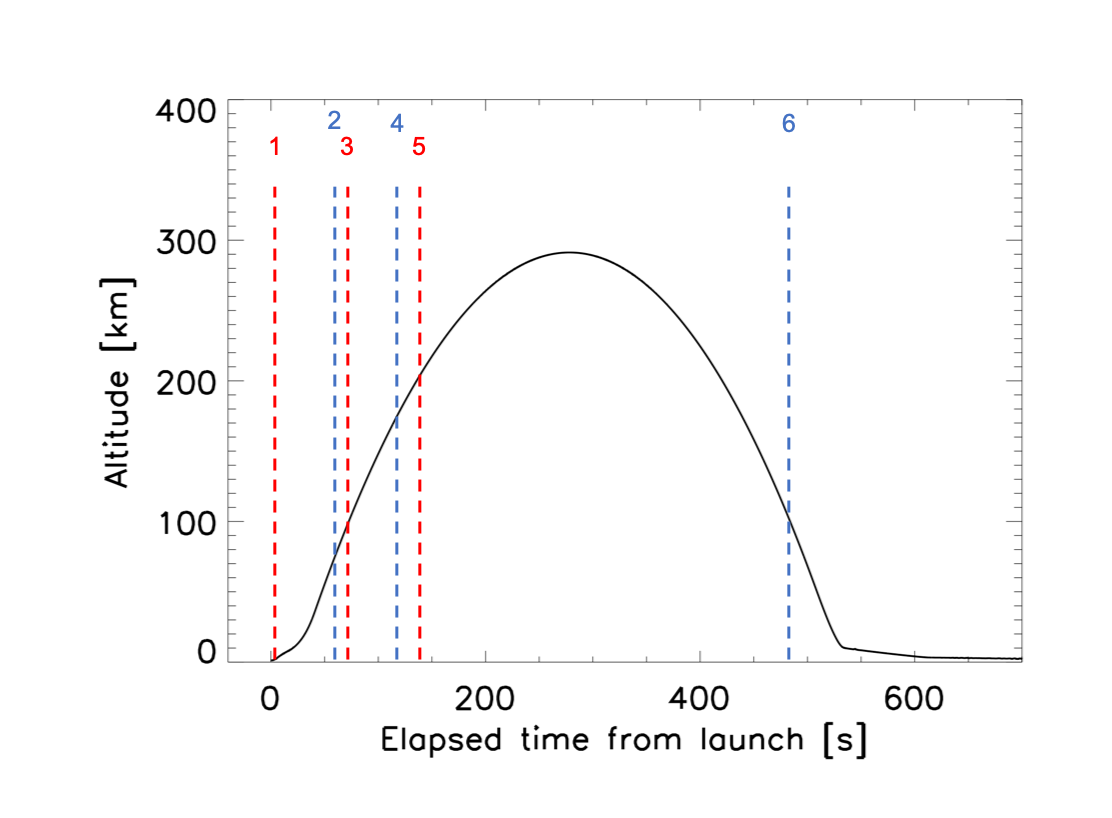
\includegraphics[width=0.7\textwidth]{figures/altevents.png}
\caption{The altitude of the ESIS rocket determined from White Sands Missile Range radar data as a function of elapsed time from launch.  The event times listed in Table~\ref{tab:timeline} are labeled.}
\label{fig:timeline}
\end{center}
\end{figure}


\subsection{Pointing} \label{sec:point}

To determine the roll offset and absolute pointing post flight, the AIA\,304\,\AA\ image taken at ???~UT was used as a reference against the ESIS images taken at ???~UT.  The roll offset, found to be \change{$\sim0.???\pm 0.005^\circ$} (clockwise about Sun center), is within the tolerances for SPARCS pointing.  Figure~\ref{fig:fov} shows the full-disk AIA\,304\,\AA\ image. The ESIS FOV is indicated by the octagon.  

\begin{figure}[h!]
\begin{center}
\includegraphics[width=0.7\textwidth]{}
\caption{The reference AIA 304\,\AA\ data taken at ???~UT, which was used for determining the absolute pointing. The octagon indicates the ESIS FOV.}
\label{fig:fov}
\end{center}
\end{figure}

\begin{center}
\begin{table}[H]
\caption{ESIS Flight Data Summary (*Solar coordinates; solar north at top of frame.)}
\begin{tabular}{ll | l l}\hline
Wavelength Range &   ???\,\AA\  & Image Size  & 2064$\times$1024\\
Launch Date & September 30, 2019 & Field of View  & ?\arcmin octagonal \\
Data Acquisition Time & ??? - ??? & Pointing  & (-?\arcsec, ?\arcsec)\change{$\pm .3\arcsec$}  \\
Camera Gain &   [4 cameras]\change{$2.5 \pm 0.02$}\,elec DN$^{-1}$ & Roll & \change{$??? \pm ???^\circ$ CW} \\
Camera Noise*: & & Exposure Time & 10\,s\\
\hspace{0.2in}NE Quad & [?,?,?,?] DN & Light Data Set: &\\
\hspace{0.2in}NW Quad & [?,?,?,?] DN & \hspace{0.2in}No. of Images & 29\\
\hspace{0.2in}SE Quad  & [?,?,?,?] DN & &\\
\hspace{0.2in}SW Quad  & [?,?,?,?] DN & Dark Data Set & \\
Plate Scale  & 0.??\arcsec\ pixel$^{-1}$ &  \hspace{0.2in}No. of Images & ? \\
\hline
\end{tabular}
\label{tab:data_info}
\end{table}
\end{center}


	
\section{Data}
    ESIS gathers an image in each of its four detectors (channels) during every exposure.  
    Each channel has it's own grating and detector and is located around the m = 1 circle in 45 degree increments. (\textbf{also a poor way to say this}
    
    \begin{figure}
        \centering
        \includegraphics{}
        \caption{Raw CCD Data}
        \label{fig:Level0}
    \end{figure}
    
    We have broken our data prep/analysis pipeline into multiple levels, labeled one through four.
    Level 1 data prepares raw CCD data for scientific work through a quadrant dependant bias subtraction and gain correction, as well as dark subtraction and despiking (optional).
    Level 2 data adds additional meta data to the Level 1 data, including a non-linear and wavelength dependent mapping from detector to field stop for use in inversions (work in progress) \rts{This actually kinda works right now}.
    Level 3 data takes a cropped single wavelength from Level 1 data and maps to the sky plane via a non-linear, but wavelength independent mapping.
    And lastly Level 4 represents an inverted data product in the form of an [x, y , $\lambda$] cube (\textbf{probably a better way to write this}), the end goal of the ESIS instrument.
    Below each complete data level is explored in more detail.
    
    \subsection{Level 1 Data}
    
        The Level-1 dataset is a sequence of images derived from the Level-0 (raw) dataset.
        The images in this dataset have had camera-level effects such as pedestal, gain, and dark current removed.
        Also, the images in this dataset have had the 
        Camera-level effects such as pedestal, gain, dark current, and light-insensitive pixels have been removed from the images in this dataset.
        The images 
        This dataset removes camera-level effects from the Level-0 dataset such as pedastal, gain, dark current and light-insensitive pixels (such as overscan pixels).
        
        
        Also, Level-1 images have the light-insensitive pixels (such as the overscan pixels) removed 
    
        The goals of the Level-1 dataset are to remove camera-level effects (pedestal, gain, and dark current), trim light insensitive pixels, and to remove spikes. to prepare for the images for coalignment.
    
        \begin{itemize}
            \item Bias Subtraction
            \item Gain Correction
         
            
                 Get in touch with MSFC about different apparent channel gains.
            \item Dark Subtraction
            \item Despiking
        \end{itemize}
       Raw ESIS data (Figure \ref{fig:Level0}) must first be corrected for quadrant dependant gain and bias, have overscan and blank pixels removed, and be dark subtracted prior to further analysis.
       
	       


    \subsection{Level 3 Data}
        \begin{itemize}
            \item Co-Alignment to AIA 304
            \item Quadratic Internal Alignment
            \item Vignetting Correction
            \item Conversion to Photons
        \end{itemize}
        
        The ESIS Level 3 data product was created to provide a co-aligned, single wavelength image in each channel for quicker identification of events with non-zero LOS velocities, and easier comparison with coordinated data that don't require inversion. 
        It will also allow for single wavelength inversion with assumptions prior to the completion of a more complete optical distortion model. 
        A quick method for identifying solar events with significant velocity is by taking the difference between two ESIS channels.
        Each ESIS channel disperses features with non-zero LOS velocities a different direction, determined by the asymuthal position of each grating. 
        Stationary solar features will have the same presentation in each camera and moving features will be smeared in different directions.
        Therefore, significant differences between ESIS images, for a given wavelength, highlight bright solar features with significant velocity.
        
        The four ESIS channels were spatially co-aligned in two steps.  
        First, each ESIS image is cropped around the desired spectral and then co-aligned to the closest AIA 304 image in time.  
        AIA 304 was chosen because, despite a formation temperature difference, it is the AIA EUV channel most visually similar to O V, in background and bright events.
        The co-alignment was achieved through a linear transformation of the cropped ESIS image that maximizes the zero lag cross-correlation between it and AIA 304.
        Despite each image being in a different wavelengths we found normalized peak zero lag cross-correlations around .9 (\textbf{PULLING THIS NUMBER OUT OF MY ASS FOR NOW, BUT IT'S CLOSE.})
        After this step each ESIS channel has been re-binned to AIA resolution and can be assigned WCS information based on AIA Level 1.5 (\textbf{ADD NOTES ABOUT STANDARD AIA PREP Above)}.
        Since ESIS has a slightly non-linear distortion function \citep{ESIS}, an additional internal alignment step is performed.
        Choosing a single ESIS channel as reference, in our case Camera 1, each other camera is co-aligned to it via a quadratic transformation that maximizes the zero-lag cross-correlation between it and the reference channel.
        After performing this additional internal alignment we find that not only is the zero-lag cross-correlation between each channel and the reference channel improved, but also the cross correlation between each combination of channels.
        
        \textbf{Time for a Figure.}
        
        In order to use Level 3 data for early inversion the intensity needs to normalized between channels and converted to photons to properly account for uncertainty.
        Since each ESIS CCD has a quadrant specific gain \citep{ESIS}, the conversion from DN to photon is done to Level 1 data prior to co-alignment efforts.
        The wavelength used when converting to photons corresponds to the spectral line cropped out of Level 1 prior to co-alignment.
        Each ESIS channel has a linear trend in intensity along the dispersion direction due to internal vignetting in the optical system \citep{ESIS}.
        This linear trend in the background is apparent in difference images that haven't been corrected.
        
        \textbf{Figure, Show Corrected and Uncorrected?}
        
        To correct the trend, we divide out a linear trending background from each image with a slope oriented to the dispersion direction in each channel, each with a different slope.
        The vignetting field divided out for each channel is,
            \begin{equation}
                \label{eqn:vignet}
                V(\alpha) = 
            \end{equation}
        
        The slope of each background is a free parameter in our fit.
        For each of the four ESIS channels we mask off the portion common to them all with no contribution from Mg X (\textbf{wavelength?}).
        The four channels of ESIS give 6 possible difference images for fitting the vignetting function. 
        For each difference image we take a mean of each column and fit a line to it as a function of column position.
        When the average slope of all six fits is minimized we consider the vignetting corrected. 
        
        
        [Copied from Hi-C paper as a reminder that we need to talk about atmospheric absorption somewhere.] We use the normalized total intensities of the Level~1.0 processed flight data (processing levels described in Section~\ref{sec:data}) to assess the relative atmospheric absorption of the signal as a function of flight time.  The transmission, shown in Figure~\ref{fig:absorb} in combination with the payload altitude, is calculated as the inverse of the relative absorption (i.e., (absorption coefficient)$^{-1}$). More than 4 minutes of data were unaffected by the atmosphere.  The atmospheric absorption was compensated for in the Level~1.5 processed data set by multiplying the images by their respective absorption coefficient.  These coefficients are provided in the header of this processed set.
        
        
        A summary of the flight data parameters, as described in the preceding sections, is provided below in Table~\ref{tab:data_info}. 



\section{Events}
    \subsection{Explosive Events}
        \begin{itemize}
            \item Quantity, Spatial and Temporal Scale
            \item Burstiness 
        \end{itemize}
    
    \subsection{Main Event}

\section{Discussion/Conclusions and Future Work}

